\documentclass[crop,tikz]{standalone}
\usetikzlibrary{backgrounds}
\colorlet{blue}{cyan}
\tikzset{
  inverted/.style = {
    color=white,
    background rectangle/.style={fill},
    show background rectangle
  }
}
\usepackage{pgfplots}
\pgfplotsset{compat=1.13}

% Field lines and lines of constant potential for an electric dipole.
%
% Inspired by the expressions given in Fritsche, "Grundkurs
% Funktionentheorie", section 1.5.8, example C.

\pgfplotsset{
  inverted/.style = {
    every axis legend/.append style={
      draw=white,
      fill=black,
      text=white
    }
  },
  every non boxed x axis/.append style={
    axis line style={-latex}
  },
  every non boxed y axis/.append style={
    axis line style={-latex}
  }
}

\begin{document}

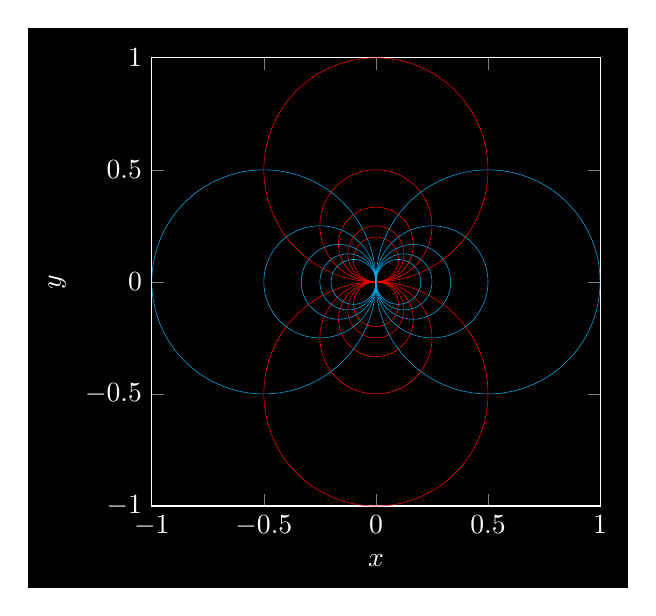
\begin{tikzpicture}[inverted,inverted]
  \pgfmathsetmacro{\numberoffieldlines}{10};
  \pgfmathsetmacro{\numberofpotentiallines}{10};
  \pgfmathsetmacro{\chargepos}{0.1};
  \pgfmathsetmacro{\remin}{-1};
  \pgfmathsetmacro{\remax}{-\remin};
  \pgfmathsetmacro{\immin}{-1};
  \pgfmathsetmacro{\immax}{-\immin};
  \begin{axis}[inverted,
    axis equal image,
    xmin={\remin}, xmax={\remax},
    ymin={\immin}, ymax={\immax},
    xlabel={$x$},
    ylabel={$y$},
    samples=100,
    domain=0:360,
    declare function = {
      Er(\c) = 1/(2*\c);
      Ex(\x,\c) = Er(\c)*cos(\x);
      Ey(\x,\c) = Er(\c)*sin(\x) - 1/(2*\c);
      phir(\c) = 1/(2*\c);
      phix(\x,\c) = phir(\c)*cos(\x) + 1/(2*\c);
      phiy(\x,\c) = phir(\c)*sin(\x);
    },
    ]
    % field lines
    \pgfplotsinvokeforeach{{-\numberoffieldlines/2},...,{\numberoffieldlines/2}}{
      \addplot[red,very thin] ({Ex(x,#1)}, {Ey(x,#1)});
    }
    % lines of constant potential
    \pgfplotsinvokeforeach{{-\numberofpotentiallines/2},...,{\numberofpotentiallines/2}}{
      \addplot[blue,very thin] ({phix(x,#1)}, {phiy(x,#1)});
    }
  \end{axis}
\end{tikzpicture}
\end{document}
